\def\pathToRoot{.}
\documentclass[a4paper, 12pt]{article}

\usepackage[utf8]{inputenc}
\usepackage{ifthen}
\usepackage{xparse}
\usepackage{scrextend}
\usepackage{setspace}
\usepackage{verbatim}
\usepackage{color}
\usepackage[inline]{enumitem}
\usepackage[colorlinks=true, linkcolor=black, citecolor=black]{hyperref}

\usepackage{tikz}
\usepackage{pgfplots}
\usepackage{bbold}
\usepackage{listings}

\usepackage{subcaption}

\usepackage{amsmath}
\usepackage{amssymb}
\usepackage{latexsym}
\usepackage{hyperref}
\usepackage{cleveref}

\definecolor{gray}{rgb}{0.2,0.2,0.2}

\pagenumbering{arabic}


\usepackage[a4paper, left=2cm, top=2cm, right=2cm, bottom=2cm]{geometry}

\usepackage{multirow}
\usepackage{fancyvrb}

\newcommand{\vect}[1]{\boldsymbol{#1}}

\newcounter{exerciseCounter}
\setcounter{exerciseCounter}{0}

\newcommand{\exerciseNumber}{\sheetnumber.\arabic{exerciseCounter}}

\setenumerate{label=\alph*)}

% Sheet Header
\newcommand{\exercisehead}[3]
{
    \def\sheetnumber{#1}
    \begin{center}
        \begin{minipage}{0.45\linewidth}
            \textsc{Universität des Saarlandes}
            \par
           Prof. Dr. Dietrich  Klakow
           \par
           Lehrstuhl für Signalverarbeitung
           \par
           NNIA Winter Term 2019/2020
        \end{minipage}
        \begin{minipage}{0.45\linewidth}
            \begin{flushright}
               
\includegraphics[width=0.30\linewidth]{headers/lsv_logo.jpg}
            \end{flushright}
        \end{minipage}
        \vspace{5pt}
        \hrule
        \vspace{12pt}
        \doublespacing
        {
            \LARGE
            \textbf{Exercise Sheet #1}
        }
        \par
        {
            \large
            #2
        }
        \par
        \ifdefined\issolution
        \textit{(Solutions)}
        \else
        \fi
        
    \textbf{Deadline: #3}

    \end{center}
    \vspace{2pt}
    \hrule
    \vspace{12pt}
}

% Exercise environment
\NewDocumentEnvironment{exercise}{oo}
{
	\refstepcounter{exerciseCounter}
	\par
	\vspace{12pt}
    \noindent
    \textbf{Exercise \exerciseNumber \  - #1}\IfNoValueF{#2}{\hfill(#2 points)}
	\vspace{12pt}
	\par
	\begin{addmargin}[12pt]{0pt}
}
{
    
	\end{addmargin}
	\par
	\vspace{12pt}
}

% Solution environment
\newenvironment{solution}
{
		\ifthenelse{\isundefined{\issolution}}
		{
			\comment
		}
		{
			\par
			\color{gray}
			\vspace{6pt}
			\textit{Solution \exerciseNumber}
			\par
			\begin{addmargin}[30pt]{0pt}
		}
}
{
		\ifthenelse{\isundefined{\issolution}}
		{
		}
		{
			\end{addmargin}
			\par
			\vspace{12pt}
		}
}



\def\issolution{}

\begin{document}

% {Sheet number}{headline}{deadline}
\exercisehead{6}{\small Philip Georgis [s8phgeor], Pauline Sander [s8pasand], Vilém Zouhar [vizo00001] }{5.1.2020}

\section*{Exercises}


\begin{exercise}[Network scheme]

%We make use of the following two matricies to simplify the expressions (to avoid cases).
\textbf{Definitions:} \\
    $\textbf{X} \in \mathbf{R}^{nx3}$ contains the input data (\textit{age}, \textit{class}, \textit{survived})\\
    $\textbf{y} \in \mathbf{R}^{nx1}$ contains the \textit{ticket prices} \\
    $\textbf{b} \in 1^{nx1}$ a bias vector of ones (only one because they have the same shape for both layers) \\
    $\textbf{W}^{(1)} \in [0,1]^{4x4}$ weight matrix mapping from input to hidden layer \\
    $\textbf{W}^{(2)} \in [0,1]^{5x1}$ weight matrix mapping from hidden to output layer \\
    %J^{n,k} = [(0, 0, \ldots, 0, 1)^T]^{(n\times 1)} \times [(1, 1, \ldots, 1)]^{(1\times k)} \qquad \textit{only bottom-most row} \\
    concat(\textbf{X},\textbf{y}) - operation that appends vector \textbf{y} as a column to matrix \textbf{X} \\ \linebreak
\textbf{Formula:}    
\begin{align}
\hat{y} = \textbf{e}\footnotemark & = concat( ReLU(concat(\textbf{X},\textbf{b}) \times \textbf{W}^{(1)}), \textbf{b}) \times \textbf{W}^{(2)} \\
Loss = \textbf{L} & = MSE(\hat{y}, \textbf{y}) \\
& = \frac{1}{n} \sum^n \Bigg(concat( ReLU(concat(\textbf{X}_n,\textbf{b}_n) \times \textbf{W}^{(1)}_n), \textbf{b}_n) \times \textbf{W}^{(2)}_n - \textbf{y}_n \Bigg)^2
\end{align}
\footnotetext{This is the name in the computational graph in exercise 6.2.}
This gives us the following network scheme (see next page):
\begin{figure}
    \centering
    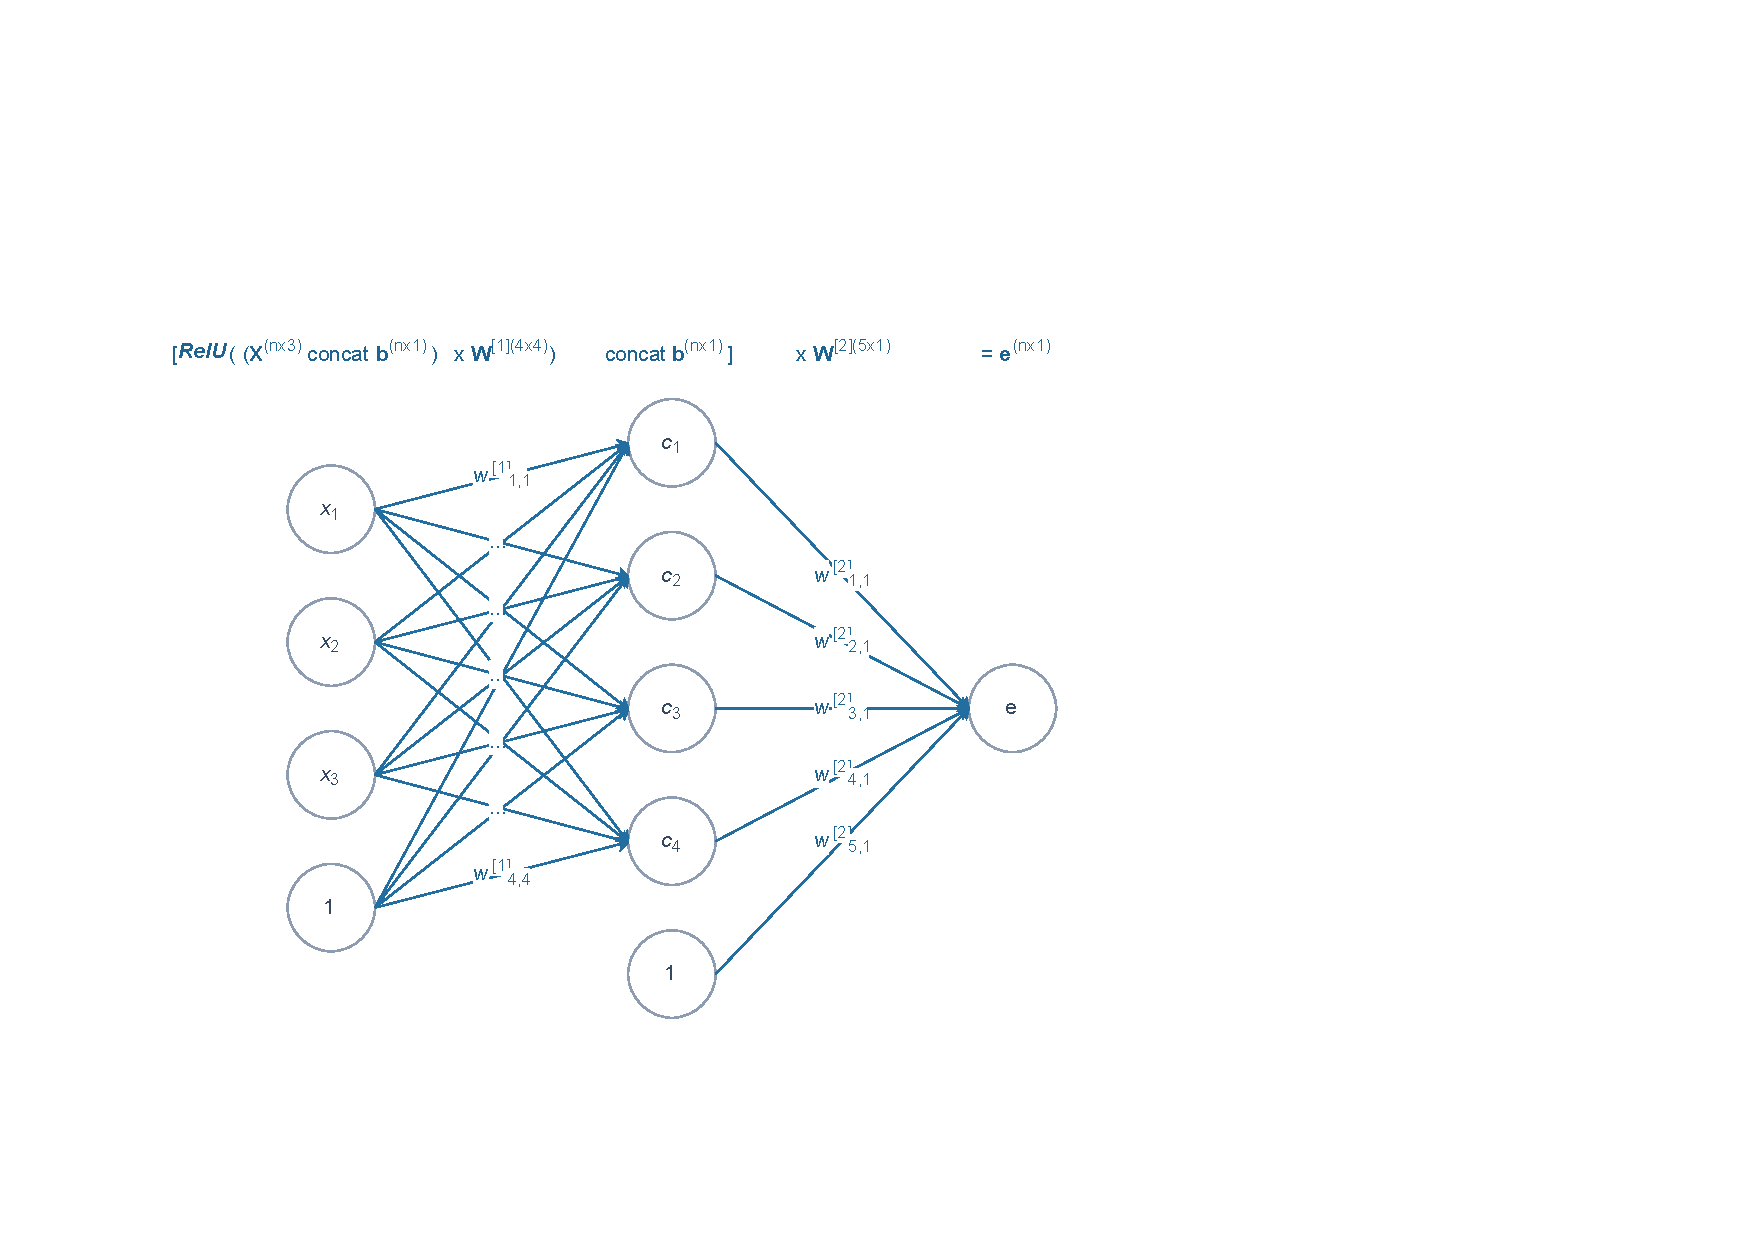
\includegraphics{img/Network_scheme.pdf}
    \caption{Network scheme}
    \label{fig:my_label}
\end{figure}
\end{exercise}
\pagebreak

\begin{exercise}[Computation graph]

\begin{figure}[ht!]
    \centering
    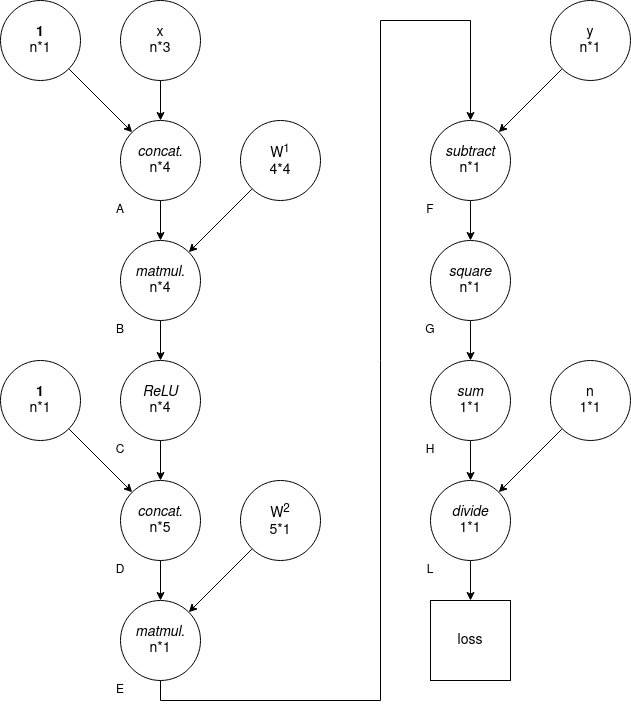
\includegraphics[width=0.8\linewidth]{img/comp_graph.png}
\end{figure}

\end{exercise}

\clearpage

\begin{exercise}[Backpropagate]

Biases are simply part of the weight matrices. The forward propagation is vectorized.

\newcommand{\starchen}{\qquad \star}

\begingroup
\allowdisplaybreaks
Forward pass:
\begin{align*}
% forward computation
L^{(1x1)} = \frac{H}{n} \qquad & \\
H^{(1x1)} = \sum_{k=1}^n G_{k} \qquad & \\
G_k^{(1x1)} = F_k^2 \qquad & \\
F^{(nx1)} = E - \textbf{y}^{nx1} \qquad & \qquad = concat( ReLU(concat(\textbf{X},\textbf{b}) \times \textbf{W}^{(1)}), \textbf{b}) \times \textbf{W}^{(2)} - \textbf{y}\\
E^{(nx1)} = D \times W^{(2)(5x1)} \qquad & \qquad = concat( ReLU(concat(\textbf{X},\textbf{b}) \times \textbf{W}^{(1)}), \textbf{b}) \times \textbf{W}^{(2)} \\
D^{(nx5)} = concat(C,\textbf{b}) \qquad & \qquad = concat( ReLU(concat(\textbf{X},\textbf{b}) \times \textbf{W}^{(1)}), \textbf{b})\\
C^{(nx4)} = ReLU(B)  \qquad & \qquad  = ReLU(concat(\textbf{X},\textbf{b}) \times \textbf{W}^{(1)})\\
B^{(nx4)} = A \times W^{(1)(4x4)} \qquad & \qquad = concat(\textbf{X},\textbf{b}) \times W^{(1)}\\
A^{(nx4)} = concat(\textbf{X},\textbf{b}) \qquad & \\
\end{align*}

Backpropagation $W^{(2)}$
\begin{align*}
& \frac{\partial L}{\partial W^{(2)}} = \frac{\partial L}{\partial H} \frac{\partial H}{\partial G} \frac{\partial G}{\partial F} \frac{\partial F}{\partial E} \frac{\partial E}{\partial w^{(2)}_{j}} \\
& \frac{\partial L}{\partial H} = \frac{1}{n}  \\
& \frac{\partial H}{\partial G} = \sum^n \\
& \frac{\partial G}{\partial F} = 2 \cdot F^{(nx1)} = 2 F^{T(1xn)} \\
& \frac{\partial F}{\partial E} = 1 \\
& \frac{\partial E}{\partial W^{(2)}} = D \\
& \Rightarrow \frac{\partial L}{\partial W^{(2)}} = \frac{1}{n} \sum^n [2 \cdot F^{T(1xn)} \cdot 1 \cdot D^{(nx5)}] = \frac{2}{n} \sum[F^T D]^{(1x5)} = \frac{2}{n} F^T D \\
& \Rightarrow \frac{2}{n} (\hat{y} - y)^{T(1\times n)} \Bigg[ concat( ReLU(concat(\textbf{X},\textbf{b}) \times \textbf{W}^{(1)}), \textbf{b}) \Bigg]^{(n\times 5)}
\end{align*}

Backpropagation $w^{(1)}_{i,j}$
\begin{align*}
& \frac{\partial L}{\partial w^{(1)}_{i,j}} = \frac{\partial L}{\partial H} \frac{\partial H}{\partial G} \frac{\partial G}{\partial F} \frac{\partial F}{\partial E} \frac{\partial E}{\partial D} \frac{\partial D}{\partial C} \frac{\partial C}{\partial B_{i,j}} \frac{\partial B_{i,j}}{\partial w^{(1)}_{i,j}} \\
& \frac{\partial E}{\partial D} = W^{(2)} \\
& \frac{\partial D}{\partial C} = this does not work \\
& \frac{\partial C}{\partial B_{ij}} = R'(B)_{ij} = \begin{cases}
    1 \hspace{0.3cm} B_{ij} > 0\\ %\, \wedge\, i = j  \\
    0 \hspace{0.3cm} \text{else} \\
\end{cases} \\
& \frac{\partial B_{ij}}{\partial w^{(1)}_{ij}} = A_{ij} \\
& \Rightarrow \frac{\partial L}{\partial W^{(1)}} = \\
& = \frac{1}{n} \sum_{k=1}^n \Bigg[ \bigg[  [ 2 \cdot F \times 1 \times (W^{(2)})^T] \times I^4\bigg] \odot R'(B) \Bigg]_{k,*} \times A_{k,*} \\
& = \frac{2}{n} A^T \Bigg[ \bigg[ F \times (W^{(2)})^T \times I^4\bigg] \odot R'(B) \Bigg] \\
& \Rightarrow \frac{2}{n} (x + J^{n,4})^{T, (4\times n)} \Bigg[ \bigg[ (\hat{y} - y) \times (W^{(2)})^T \times I^4\bigg]^{(n\times 4)} \odot R'\big((x+J^{n,4}) \times W^{(1)}\big)^{(n\times 4)} \Bigg]^{(n\times 4)}
\end{align*}
\endgroup

% old solution
% \begingroup
% \allowdisplaybreaks
% \begin{align*}
% % L
% &  \frac{\partial L}{\partial L} = 1 & & \starchen\\
% % H
% & L = \frac{H}{n} & \frac{\partial L}{\partial H} = \frac{1}{n} & \starchen \\
% % G
% & H = \sum_i^n G_{i,1} & \frac{\partial H}{\partial G_i} = 1 &  \\
% & \frac{\partial L}{\partial G} = \frac{\partial L}{\partial H} \cdot \frac{\partial H}{\partial G} & = \frac{1}{n} \cdot \sum^n 1 & \starchen \\
% % F
% & G_i = F_i^2 & \frac{\partial G_i}{\partial F_i} = 2\cdot F_i & \\
% & \frac{\partial L}{\partial F} = \frac{\partial L}{\partial G} \cdot \frac{\partial G}{\partial F} & = \frac{2}{n} \sum^n_k F_k & \starchen \\
% % E
% & F_i = E_i - y_i & \frac{\partial F}{\partial E} = \mathbf{I}_{(n\times n)} & \\
% & \frac{\partial L}{\partial E} = \frac{\partial L}{\partial F} \cdot \frac{\partial F}{\partial E} & = \frac{2}{n} F \times \mathbf{I}_{(n\times n)} = \frac{2}{n} \sum^n_k F_k & \starchen \\
% % W2
% & E = D \times W^{(2)} & \frac{\partial E}{\partial W^{(2)}} = D & \\
% & \frac{\partial L}{\partial W^{(2)}} = \frac{\partial L}{\partial E} \cdot \frac{\partial E}{\partial W^{(2)}} & = \frac{2}{n} \sum^n_k F_k \times D_{k*} & \starchen \\
% % D
% & \frac{\partial E}{\partial D} = (W^{(2)})^T & \\
% & \frac{\partial L}{\partial D} = \frac{\partial L}{\partial E} \cdot \frac{\partial E}{\partial D} & = \frac{2}{n} \cdot F \times (W^{(2)})^T & \starchen \\
% % C
% & D_{ij} = \begin{cases}
%     C_{ij} \qquad j \in \{1, 2, 3, 4 \} \\
%     1 \hspace{0.35cm} \qquad j = 5 \\
% \end{cases} & \frac{\partial D}{\partial C} = \mathbf{I}_{(5\times 5)} - \mathbf{1}_5 \times \mathbf{1}_5^T & \\
% & \frac{\partial L}{\partial C} = \frac{\partial L}{\partial D} \cdot \frac{\partial D}{\partial C} & = \frac{2}{n} \cdot [F \times (W^{(2)})^T]^{(n\times 4)} \ \textit{(last column dropped)} & \starchen \\
% % B
% & C_{ij} = \begin{cases}
%     B_{ij} \qquad B_{ij} > 0  \\
%     0 \hspace{0.35cm} \qquad \text{else} \\
% \end{cases}
% & R'(B)_{ij} = \frac{\partial C_{ij}}{\partial B_{ij}} = \begin{cases}
%     1 \hspace{0.3cm} B_{ij} > 0  \\
%     0 \hspace{0.3cm} \text{else} \\
% \end{cases} & \\
% & \frac{\partial L}{\partial B} = \frac{\partial L}{\partial C} \cdot \frac{\partial C}{\partial B} & = \frac{2}{n} \cdot [F \times (W^{(2)})^T]^{(n\times 4)}\odot R'(B) & \starchen \\
% % W1
% & B = A \times W^{(1)} & \frac{\partial B}{\partial W^{(1)}} = A^T & & \\
% & \frac{\partial L}{\partial W^{(1)}} = \frac{\partial L}{\partial B} \cdot \frac{\partial B}{\partial W^{(1)}} & = \frac{2}{n} \cdot \sum^n_k \big[[F \times (W^{(2)})^T]^{(n\times 4)})_{k*} \odot R'(B)\big] \times A^T_{k*} & \starchen
% \end{align*}
% \endgroup

\end{exercise}


\begin{exercise}[PyTorch]
Tensors are smart objects and the operations on them also produce the gradient and can track history. The partial gradient then has to be defined by the operation. The autograd then constructs a dynamic computational graph, which is an acyclic connected graph from this node with leaves as the input vectors. It is invoked using \texttt{backward}.
\end{exercise}

\end{document}
